% easychair.tex,v 3.5 2017/03/15

\documentclass{easychair}
%\documentclass[EPiC]{easychair}
%\documentclass[EPiCempty]{easychair}
%\documentclass[debug]{easychair}
%\documentclass[verbose]{easychair}
%\documentclass[notimes]{easychair}
%\documentclass[withtimes]{easychair}
%\documentclass[a4paper]{easychair}
%\documentclass[letterpaper]{easychair}

\usepackage{doc}
%\usepackage{amsmath}

% use this if you have a long article and want to create an index
% \usepackage{makeidx}

% In order to save space or manage large tables or figures in a
% landcape-like text, you can use the rotating and pdflscape
% packages. Uncomment the desired from the below.
%
% \usepackage{rotating}
% \usepackage{pdflscape}

% Some of our commands for this guide.
%
\newcommand{\CBCTT}{CB-CTT}
\newcommand{\UP}{UP}
\newcommand{\ASP}{ASP}
\newcommand{\clingo}{\textit{clingo}}
\newcommand{\naf}{\textit{not }} 
\newcommand{\head}{\textit{head}}
\newcommand{\body}{\textit{body}}

%\makeindex

%% Front Matter
%%
% Regular title as in the article class.
%
\title{AI-Based Tool for Curriculum-Based Course Timetabling of University of Potsdam}

% Authors are joined by \and. Their affiliations are given by \inst, which indexes
% into the list defined using \institute
%
\author{
Christian Dohrmann 
\and
Ulrike Lucke 
\and
Torsten Schaub 
\and 
Sebastian Schellhorn 
}

% Institutes for affiliations are also joined by \and,
\institute{
  University of Potsdam,
  Germany\\
  \email{\{christian.dohrmann, ulrike.lucke, torsten.schaub, sebastian.schellhorn\}@uni-potsdam.de}
 }

%  \authorrunning{} has to be set for the shorter version of the authors' names;
% otherwise a warning will be rendered in the running heads. When processed by
% EasyChair, this command is mandatory: a document without \authorrunning
% will be rejected by EasyChair

\authorrunning{Dohrmann et al.}

% \titlerunning{} has to be set to either the main title or its shorter
% version for the running heads. When processed by
% EasyChair, this command is mandatory: a document without \titlerunning
% will be rejected by EasyChair
\titlerunning{AI-Based Tool for \CBCTT{} of \UP{}}

\begin{document}

\maketitle

\begin{abstract}
  \begin{itemize}%
    \item%
    Education is a fundamental part of universities and comes together with the time consuming non-trivial task of finding suited timetables for teaching. 
    \item%
    The corresponding problem is called Curriculum-Based Course Timetabling and considers possible constraints when looking for a conflict free timetable.
    \item% 
    We addressed this problem by following a knowledge representation and reasoning approach, describing constraints and possible assignments of courses to time slots. 
    \item% 
    Possible assignments are collected by a prototype webinterface and corresponding constraints are respected by finding automatically a timetable using an AI. 
    \item%  
    We discuss resolved redundancies, saved time and possible future benefits, when comparing traditional and new approach regarding needs of University of Potsdam. 
  \end{itemize}%
\end{abstract}

% The table of contents below is added for your convenience. Please do not use
% the table of contents if you are preparing your paper for publication in the
% EPiC Series or Kalpa Publications series

%\setcounter{tocdepth}{2}
%{\small
%\tableofcontents}

%\section{To mention}
%
%Processing in EasyChair - number of pages.
%
%Examples of how EasyChair processes papers. Caveats (replacement of EC
%class, errors).

%------------------------------------------------------------------------------
\section{Motivation}
\label{sec:motivation}

\begin{itemize}%
  \item% 
  Education is a fundamental part of universities, usually addressed by offering a variety of courses may containing lectures, exercises, seminars, projects, etc. within a defined study program. 
  \item% 
  In order to obtain optimal timetables, all offered courses must be assigned to a time slot and room, respecting some constraints. 
  \item%
  A time slot is a combination of a day and a time.  
  \item%
  The corresponding problem is called Curriculum-Based Course Timetabling (\CBCTT{}; \cite{becaroto15}) and considers possible constraints when looking for a conflict free timetable. 
  \item%
  A solution to a \CBCTT{} problem is an assignment of courses to time slots and rooms, such that each corresponding hard constraint is satisfied. 
  \item% 
  An optimal solution is a solution with minimal penalty regarding soft constraints. 
  \item% 
  Traditionally, such \CBCTT{} problems are solved by humans and involving a lot of time and agreements. 
  \item% 
  Especially, when several people are involved to develop timetables, redundancies and conflicts among resulting plans may caused. 
  \item% 
  In addition, obtained timetables are often not proved to be optimal and possibly violate soft or hard constraints. 
  \item% 
  In our work, we model corresponding soft and hard constraints in context of University of Potsdam (\UP{}), to get conflict free and optimal timetables derived by an AI. 
  \item%
  Thanks to its simple modeling language and high performance solving capabilities, Answer Set Programming (\ASP{}; \cite{baral02a}) is a well suited approach of knowledge representation and reasoning to model \CBCTT{} problems, as \cite{bainkaokscsotawa18a} showed.
  \item% 
  We developed a prototype webinterface allowing planners and lecturers to enter availabilities of teaching times and suited rooms regarding courses, to find during a couple of seconds automatically a timetable provably respecting needed constraints among curricula. 
  \item% 
  By comparing the new and traditional approach, we illustrate resolved redundancies, saved time and possible future benefits. 
\end{itemize}%


%------------------------------------------------------------------------------
\section{Approach}
\label{sec:approach}

\begin{itemize}% 
  \item% 
  In the following, we describe the traditional and new approach of finding a timetable and link it to the course catalog at \UP{}. 
  \item% 
  To this end, let us first describe the structure and relation among curricula, modules, examination tasks and courses. 
  \item%
  A cohort of students is given by a corresponding program and semester wrt the curriculum. 
  \item% 
  Each curriculum is defined by referring to modules needed to be accomplished. 
  \item% 
  Modules define the number and type of courses and course components as well as their secondary and primary examination tasks. 
  \item%
  For simplicity, in the following we refer courses and course components by courses and make explicit when needed. 
  \item% 
  Courses are linked to, possibly several, secondary and sometimes primary examination tasks of a set of modules. 
  \item%  
  Since modules are associated to possibly several curricula, the linkage of examination tasks to courses induces involved curricula and cohorts possibly participating to a course. 
  \item% 
  Whenever a module occurs in several curricula, possibly of different institutes or faculties, then the goal to find a conflict free timetable becomes more complicated. 
  \item% 
  In the traditional case, lectures with a big number of participants are planned first, due to a limited number of large lecture halls and imports/exports of courses among curricula. 
  \item% 
  The resulting timetable regarding big lectures, needs a lot of communication and agreements among several planners to ensure a conflict free timetable for involved cohorts and lecturers. 
  \item% 
  Especially, in case of degree programmes to become a teacher of allowed combinations of topics, \UP{} developed a time frame model to prevent conflicts among courses of most common combination of topics\footnote{https://www.uni-potsdam.de/en/studium/studying/organizing-your-studies/potsdams-time-frame-model}.
  \item% 
  On top of scheduled big lectures, remaining courses are planned by planners of each institute to achieve suitable timetables. 
  \item% 
  A timetable should avoid conflicts regarding multiple usage of rooms, lecturers and cohorts as well as respecting particular demands of courses, like technical equipment.
  \item% 
  A timetable becomes more optimal, if it respects for instance traveling time of consecutive courses, teaching load per day and gaps among courses of a day aiming on same cohort or lecturer, respectively. 
  \item% 
  As soon as a solution is found, each planner has to copy it course by course to universities course catalog, link each course to examination tasks of particular modules and book a room for the assigned time slot. \\
  \item% 
  Our approach aims on time consuming communication among planners and lecturers as well as redundancies when a solution was found but has to get copied to the course catalog, linked to modules and booked to rooms. 
  \item% 
  To this end, we developed a prototype webinterface allowing planners and lecturers to create courses and course components together with its module linkages, prioritized available time slots as well as rooms and relations among courses. 
  \item% 
  Four pairwise relations among courses are provided:
  \begin{itemize}
    \item two course components are not allowed to take place in parallel, e.g. obligatory lectures of same cohort
    \item two course components have to take place in parallel (same time slot, but different rooms), e.g. two groups of exercises of the same course
    \item two course components have to take place simultaneous (same time slot and room), e.g. hosting two seminars sharing major content in same room
    \item two course components have to take place consecutive, e.g. having an exercise directly after the corresponding lecture 
  \end{itemize}
  \item%
  For each course component, the webinterface allows to state the expected number of participants as well as the need of particular equipment, e.g. large board.  
  \item% 
  See figure~\ref{fig:webinterface} illustrating parts of the prototype webinterface. 
  \begin{figure}
    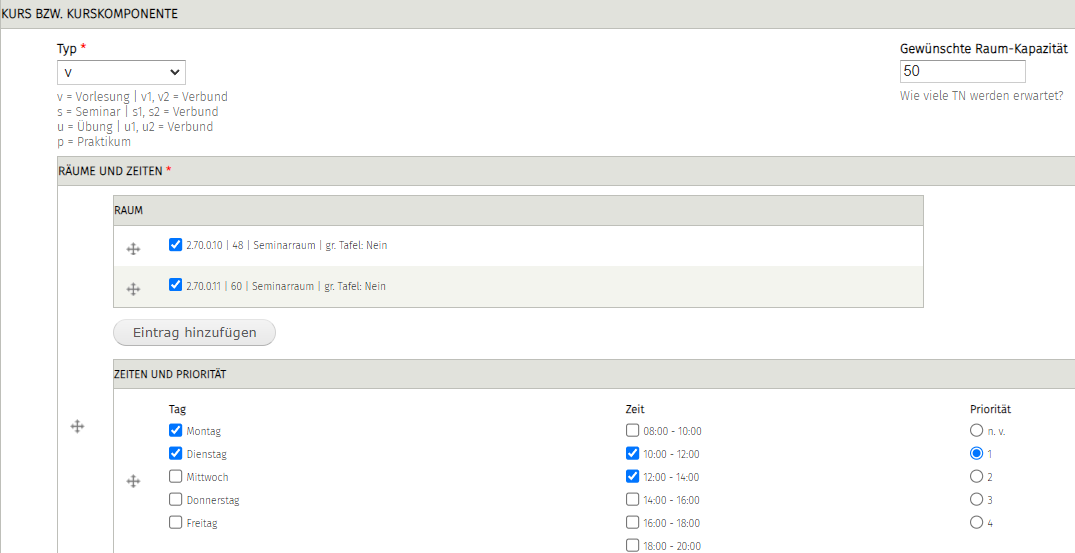
\includegraphics[width=\linewidth]{webinterface}
    \caption{Webinterface inducing availabilities by the cross product of days, times and rooms for a lecture.}
    \label{fig:webinterface}
  \end{figure}
  \item%
  The corresponding planner checks the consistence and correctness of the input data for the webinterface. 
  \item% 
  The input data together with a logic representation of necessary constraints is given to an AI, that searches for an optimal timetable. 
  \item% 
  The solution is a visualization of the resulting timetable and double checked by planners. 
  \item% 
  Note that the new approach follows the traditional idea of splitting the process into two steps, by first finding a timetable regarding big lectures and then completing it to a timetable for each institute. 
  \item% 
  The resulting timetable of each institute has to (automatically) transferred to universities course catalog respecting linked modules, time slots and rooms. 
  \item% 
  This last step of integrating the obtained timetable automatically to the course catalog is not yet part of the prototype but will omit a lot of redundancies. 
\end{itemize}%


%------------------------------------------------------------------------------
\section{\ASP{} Paradigm}
\label{sec:asp}
\begin{itemize}%
  \item% 
  \ASP{} \cite{baral02a, breitr11a} is an approach to declarative problem solving and belongs to the area of knowledge representation and reasoning. 
  \item% 
  The roots of \ASP{} go back to logic programming, nonmonotonic reasoning and constraint satisfaction \cite{gellif91a}. 
  \item% 
  The idea of \ASP{} is to describe the problem by using a formal representation, rather than telling a computer how to solve the problem. 
  \item% 
  Figure~\ref{fig:asp} illustrates this approach \cite{gekakasc12a}. 
  \begin{figure}
  \label{fig:asp}
  \begin{center}{%
    \begin{picture}(300,120)(-150,-60)
    \put(-80,+40){\makebox(0,0){\framebox(80,20){Problem}}}
    \put(-80,-40){\makebox(0,0){\framebox(80,20){Logic Program}}}
    \put(+80,+40){\makebox(0,0){\framebox(80,20){Solution}}}
    \put(+80,-40){\makebox(0,0){\framebox(80,20){Stable Models}}}
    \put(-80,+30){\vector(0,-1){60}}
    \put(-40,-40){\vector(+1,0){80}}
    \put(+80,-30){\vector(0,+1){60}}
    \put(-110,  0){\makebox(0,0){Modeling}}
    \put(+120,  0){\makebox(0,0){Interpreting}}
    \put(   0,-55){\makebox(0,0){{Solving}}}
    \end{picture}}
    \end{center}
  \caption{Declarative problem solving.}
  \end{figure}
  \item% 
  An easy and human readable modeling language \cite{cafageiakakrlemarisc19a} is used to obtain a logic program modeling the original problem. 
  \item%
  By using problem solvers like \clingo{} \cite{gekakaosscwa16a}, a solution, i.e. stable model \cite{gellif88b}, of a problem is found and has to be interpreted by the user. 
  \item% 
  Due to its simple but rich high-level modeling language as well as its elaboration-tolerance and its high-performance solving capacities, \ASP{} becomes a well suited approach to model real world problems. 
  \item% 
  The range of applications to model and solve combinatorial search problems is among planning, scheduling, configuration, probabilistic reasoning, diagnosis and repair, classification, query answering, explanation generation, multi-agent systems, natural language processing, computational biology, music composition, model checking and robotics \cite{ergele16}. 
  \item% 
  In Terms of industrial applications, \ASP{} has been used for solving (automated product) configuration \cite{soinie99a, hebasasc22a}, planning \cite{jizhkhst19a, sopobasc23a}, scheduling \cite{aldoma17a}, timetabling \cite{bainkaokscsotawa18a} and other problems \cite{fafrsctate18a}. 
  \item%
  Especially, for industrial applications, tackled by a declarative approach like \ASP{}, significant improvements wrt implementation, maintenance costs and human-machine interaction were shown. 
  \item% 
  For instance, Siemens reported to save more than 80\% of maintenance costs by using a knowledge representation and reasoning approach \cite{fafrhascsc16a}. 
\end{itemize}%

\subsection{Modeling with \ASP{}}
\label{subsec:asp}
\begin{itemize}%
  \item%
  \ASP{} provides a powerful high-level modeling language, which allows recursive definitions, default negation for dealing with the absence of information, disjunctions, aggregates, weight constraints, optimization statements and external atoms. 
  \item%
  In the following, we give a short introduction to basics of the modeling language of \ASP{} \cite{cafageiakakrlemarisc19a} and the stable models semantics of logic programs \cite{gellif88b}. \\
  \item% 
  Terms are either constants, variables, arithmetic terms or functional terms. 
  \item% 
  Constants are denoted by strings starting with lowercase letter, quoted strings or integers. 
  \item%
  Variables are denoted by strings starting with uppercase letter. 
  \item% 
  A predicate atom, is of form $p(t_1,\dots,t_n)$, where $p$ is a predicate name, $t_1,\dots,t_n$ are terms and $n\geq0$ is the arity of the predicate atom. 
  \item% 
  Predicate atoms of arity $0$ are represented by its name without parentheses.
  \item% 
  In the following, predicate atoms are called atoms for short and are denoted by $a$.
  \item% 
  An atom is called ground and can be understood as propositional, if all its variables are substituted by constants. 
  \item%
  A literal is an atom $a$ or its default negation $\naf{} a$. 
  \item% 
  Default negation, also known as negation as failure, refers to the absence of information, whereas "classical" negation induces the presence of negated information.  
  \item% 
  A rule $r$ is of form 
  \begin{align*}
    a_0 \leftarrow a_1,\dots,a_n, \naf{} a_{n+1},\dots,\naf{} a_m
  \end{align*}
  where $0\leq n\leq m$ and each $a_i$ is an atom for $1\leq i \leq m$. 
  \item% 
  Let $\head{(r)} = a_0$ and $\body{(r)} = \{a_1,\dots,a_n,\naf{} a_{n+1},\dots,\naf{} a_m\}$ the head and the body of a rule $r$, respectively. 
  \item% 
  For a set of literals $X$, let $X^+ = \{a \mid a\in X \}$ and $X^- = \{a \mid \naf{} a\in X\}$. 
  \item% 
  Intuitively, the $\head{(r)}$ of a rule $r$ must hold, if the $\body{(r)}$ holds. 
  \item% 
  The body $\body{(r)}$ of rule $r$ holds, if atoms of $\body{(r)}^+$ are provably true and atoms of $\body{(r)}^-$ are possibly false. 
  \item% 
  A rule $r$ is called fact, whenever $\body{(r)}=\emptyset$.\footnote{Usually, we drop $\leftarrow$ in this case.}  
  \item% 
  A rule $r$ is called (integrity) constraint, whenever $\head{(r)}\cap\body{(r)}^-\neq\emptyset$.%\footnote{Usually, literals $\head{(r)}$ and $\naf{} \head{(r)}$ are dropped in this case.}
  \item% 
  Integrity constraints are used to eliminate unintended solution candidates, whenever its body is satisfied. 
  \item% 
  As an example, consider rule 
  \lstinputlisting[basicstyle=\small, firstline=27, lastline=31]{example.lp}
  deriving a conflict among two course components of ``AI'' lecture and exercise that shall take place consecutive, whenever they are scheduled on different days.\footnote{In the syntax of an \ASP{} encoding `$\leftarrow$' is represented by `$:-$' and each rule terminates by a period `.'.}  
  \item%
  A logic program is a finite set of rules. 
  \item% 
  A set of ground atoms $X$ is a model of a logic program $P$, if for every $r\in P$ holds $\head{(r)}\in X$ whenever $\body{(r)}^+\subseteq X$ and $\body{(r)}^-\cap X=\emptyset$.
  \item% 
  The stable model of a program $P$ is defined relative to a set of atoms $X$, by the so called reduct $P^X$, defined by 
  \begin{align*}
    P^X=\{\head{(r)}\leftarrow \body{(r)}^+\mid r\in P, \body{(r)}^-\cap X = \emptyset\}
  \end{align*}
  \item% 
  $X$ is a stable model of a program $P$, if $X$ is the $\subseteq$-minimal model of $P^X$. 
  \item% 
  As an example consider the following program $P$
  \lstinputlisting[basicstyle=\small, numbers=left]{example.lp}
  where lines 1-21 are facts setting rooms, room capacities, course components with expected number of participants, stating ``AI'' lecture and exercise as consecutive as well as declaring possible time slots and rooms for each course component. 
  \item% 
  Line 22 sets ``AI'' lecture to time slot with identifier 42, since there is no other option. 
  \item% 
  Lines 23-26 state that either time slot with identifier 43 or 44 has to be taken for the ``AI'' exercise. 
  \item% 
  Lines 27-31 derive a conflict predicate, whenever ``AI'' lecture and exercise are not at same day and thus not consecutive. 
  \item% 
  Lines 32-33 form an integrity constraint ruling out models containing conflict predicate derived by lines 27-31. 
  \item% 
  Since atoms of lines 1-21 are facts, they belong to any model of $P$. 
  \item% 
  Let $X$ be the set containing atoms of lines 1-21. 
  \item% 
  Note that $X$ is not a model of $P$, since the body of rule in line 22 is satisfied, but not its head. 
  \item% 
  Sets 
  \begin{align*}
    X\cup&\{\texttt{book(42, ("AI", v)), book(43, ("AI", u)),} \\
         &\texttt{conflict(consecutive, ((42, ("AI", v)), (43, ("AI", u)))), conflict}\}
  \end{align*} 
  and 
  \begin{align*}
    X\cup\{\texttt{book(42, ("AI", v)), book(44, ("AI", u))}\}
  \end{align*} 
  are models of $P$, but the latter one is the only stable model of $P$. \\
  \item% 
  The basic approach of modeling a problem by an \ASP{} encoding follows a generate-and-test methodology, also known as guess-and-check, inspired by intuitions on \textit{NP} problems. 
  \item%  
  In case of \CBCTT{}, one could think of generating any timetable as a model and ruling out certain models by posing particular (hard) constraints. 
\end{itemize}%

\subsection{Modeling \CBCTT{} of \UP{}}
\label{subsec:modeling}
\begin{itemize}%
  \item% 
  Since a course may consists of several course components of possibly different types, e.g. a lecture and an exercise, we identify a course component by a unique tuple of a name and its type, e.g. lecture \textit{(``Artificial Intelligence'', v)} and exercise \textit{(``Artificial Intelligence'', u)} of Artificial Intelligence course. 
  \item%
  We modeled the following hard (H0-8) and soft (S0-13) constraints. 

  \textbf{H0.} Components: No component of a course should take place in parallel to its corresponding lecture, except if explicitly stated. 

  \textbf{H1.} Courses: One availability for each course component must be assigned to a time slot and room. 

  \textbf{H2.} Cohort: Obligatory lectures of the same cohort must be all scheduled in different time slots, except explicitly stated to take place in parallel. 

  \textbf{H3.} RoomOccupancy: Two course components cannot take place in the same room and time slot, except explicitly stated. 

  \textbf{H4.} Lecturer: Course components sharing a lecturer cannot be scheduled in parallel, except explicitly stated. 

  \textbf{H5.} NotParallel: Avoiding two course components to take place in parallel, whenever explicitly stated.

  \textbf{H6.} Parallel: Two course components have to take place in parallel, whenever explicitly stated.

  \textbf{H7.} Simultaneous: Two course components have to take place simultaneous, whenever explicitly stated.

  \textbf{H8.} Consecutive: Two course components have to be scheduled consecutive, whenever explicitly stated.

  \textbf{S0.} Availability: For each course component, try to serve prioritized availability on time slot and room. The penalty points reflecting corresponding priorities.  

  \textbf{S1.} RoomCapacity: For each course component, penalty points for the number of students that are expect to attend the course minus the number of seats in the corresponding room are imposed on each violation. 

  \textbf{S2.} Cohort: Course components addressed to the same cohort should be scheduled in different time slots, except explicitly stated to be in parallel. Each violation counts as a penalty point. 

  \textbf{S3.} Gaps: For a cohort as well as lecturer, corresponding course components should be scheduled in time slots as close as possible. The penalty regarding two courses sharing a cohort or lecturer, and a day is given by subtracting the earlier time from the later time. 

  \textbf{S4.} RoomStability: Two course components stated to be consecutive should be booked in the same room. The penalty points reflecting each violation. 

  \textbf{S5.} MaxLoad: For a cohort as well as lecturer the number of corresponding course components per day should be lower or equal to a given maximum. The penalty points reflecting the number of courses above the maximum. 

  \textbf{S6.} TravelTime: For a cohort as well as a lecturer, traveling time between rooms with two adjacent course components should be as small as possible. The penalty is reflected by the traveling time itself. 

  \textbf{S7-13.} RoomSuitability: Some course components prefer particular equipment like a large board, projector, computer, microphone, camera, media table or whiteboard. Each violation counts as a penalty point. 

  \item% 
  Note that some constraints are similar to those presented in \cite{bainkaokscsotawa18a}, others are new or modified.
  \item% 
  Due to lack of space, we drop the corresponding logic program here\footnote{The particular \ASP{} encoding representing above constraints can be found at GitHub: https://github.com/schellhorn/CBCTT-UP.}.  
  \item% 
  Optimization tries to minimize penalty points regarding above soft constraints. 
  \item%
  The system of \cite{bainkaokscsotawa18a}, reads instances of a standard input format \cite{bocegasc12a}, translates them into \ASP{} facts and assigns potentially any course to any time slot. 
  \item%
  In contrast, we used a direct modeling dedicated to constraints and needs of the \UP{}, which partially is not covered by the standard input format. 
  \item%
  As a design decision, we reduced the search space to collected availabilities only, instead of checking for all possible time slots and rooms for each course component.
\end{itemize}%


%------------------------------------------------------------------------------
\section{Results and Impact}
\label{sec:impact}
\begin{itemize}%
  \item%
  In \cite{bainkaokscsotawa18a} was shown, that treating \CBCTT{} problems by an \ASP{} based approach outperforms state of the art approaches and makes it well suited to tackle \CBCTT{} problems. 
  \item% 
  Our real world approach is still at a prototype stage and is lacking access to some data needed to apply all presented and modeled constraints. 
  \item%
  For winter 2023/24, an optimal and conflict free plan was found for about 160 courses aimed at big lecture halls of the Faculty of Science, all 90 courses of the Institute of Mathematics and 100 courses of the Institute of Computer Science, involving constraints H1, H3, H5, S0, S1 and S7 of above \ASP{} based modeling. 
  \item% 
  Analogously, for summer 2024, an optimal and conflict free plan was found involving about 200 courses and constraints H0, H1, H3, H5, H6, H7, H8, S0, S1, S4 and S7.  
  \item% 
  Solver \clingo{} was integrated to the web interface and needed about 170 seconds for winter and less than one second for summer, respectively, to solve the problem regarding the faculty. 
  \item% 
  Finding plans for the institutes took less than a second, respectively. 
  \item% 
  A major benefit of the presented AI-based approach is its fairness, transparency and elaboration tolerance. 
  \item% 
  Planners and lecturers are able to set a prioritized selection of availabilities and preferences to upcoming teaching periods, resulting in a provable conflict free timetable. 
  \item% 
  Getting a conflict free timetable for a faculty in a couple of seconds, respecting dependencies among several institutes at the same time, resolves a lot of communication overhead and conflicts of the earlier approach. 
  \item% 
  Thus, our approach gives planners already the opportunity to address their additional available time to other tasks. 
  \item% 
  As soon as the integration of the resulting timetable to the universities course catalog is done automatically, then even more redundancies are resolved and a lot more capacities become available. 
  \item% 
  Due to our current prototype state, we did not yet compare to other approaches\cite{feutrier23a} regarding performance. 
\end{itemize}%


%------------------------------------------------------------------------------
%\section{Related Work} % no time to check for it properly
%\label{sec:related}
%... 


%------------------------------------------------------------------------------
\section{Future Work}
\label{sec:future}
\begin{itemize}%
  \item% 
  For the future, we plan to involve an interface, allowing us to access data like previous course catalogues and curricula as well as their modules.
  \item% 
  Furthermore, we plan to develop an interface, allowing us to push final timetables to universities course catalog automatically. 
  \item% 
  Another, not trivial task, is to provide opportunities to the user to analyze and solve conflicts, whenever needed.  
  \item% 
  In a next step, we are going to extend the number of users and involve them in a feedback loop, to improve the usage of the system and check for additional needs. 
  \item% 
  In a long run, one could think about to add functionalities like drag and drop to take smaller changes by hand to a calculated timetable into account, preserving consistence regarding hard and soft constraints. 
  \item% 
  When establishing the mentioned workflow to get conflict free timetables, one could measure the average amount of time needed per planner using the traditional and new approach, respectively.
  \item% 
  Moreover, one could compare the quality of resulting timetables regarding desired hard and soft constraints. 
  \item% 
  Comparing quality and used time of both approaches may highlight the usage and impact of our new approach using AI of knowledge representation and reasoning. 
  \item% 
  The data about availabilities of different types of course components to several time slots, provides insights to the needs of room infrastructure. 
  \item% 
  One could think about, to possibly exploit entered availabilities and number of participants to derive location, size and quantity of needed lecture halls and seminar rooms, when plan to build new ones.
  \item% 
  Finally, our approach provides a lot potential to get rid of redundancies, save money and lift administrative planning tasks to the next level. 
\end{itemize}% 


\label{sec:bib}
\bibliographystyle{plain}
%\bibliographystyle{alpha}
%\bibliographystyle{unsrt}
%\bibliographystyle{abbrv}
\bibliography{refs}


%------------------------------------------------------------------------------
% Index
%\printindex

%------------------------------------------------------------------------------
\end{document}

